% Standalone article: no slides, generated PDFs, or local input files required.
\documentclass[11pt,a4paper]{article}
\usepackage[T1]{fontenc}
\usepackage[utf8]{inputenc}
\usepackage{lmodern}
\usepackage[margin=27mm]{geometry}
\usepackage{amsmath,amssymb,amsthm,mathtools}
\usepackage{microtype}
\usepackage{tikz}
\usetikzlibrary{arrows.meta,positioning}
\usepackage[hidelinks]{hyperref}
\hypersetup{pdftitle={The U3 inverse theorem: a detailed exposition},pdfauthor={Ferran Espuna Bertomeu}}
\newcommand{\E}{\mathbb E}
\newcommand{\T}{\mathbb R/\mathbb Z}
\newcommand{\Z}{\mathbb Z}
\newcommand{\R}{\mathbb R}
\newcommand{\C}{\mathbb C}
\newcommand{\F}{\mathbb F}
\newcommand{\Gh}{\widehat G}
\newcommand{\Bohr}{\operatorname{Bohr}}
\newcommand{\supp}{\operatorname{supp}}
\newcommand{\bb}{\mathcal B}
\newcommand{\abs}[1]{\left|#1\right|}
\newcommand{\norm}[1]{\left\|#1\right\|}
\newcommand{\poly}{\eta^{O(1)}}
\newcommand{\ipoly}{\eta^{-O(1)}}
\newcommand{\JT}[1]{\cite[#1]{JT}}
\newcommand{\GT}[1]{\cite[#1]{GT}}
\newcommand{\Green}[1]{\cite[#1]{Green}}
\newtheorem{lemma}{Lemma}[section]
\newtheorem{theorem}[lemma]{Theorem}
\theoremstyle{definition}
\newtheorem{definition}[lemma]{Definition}
\newtheorem{remark}[lemma]{Remark}
\newtheorem*{inverse}{Theorem 1.6 (Jamneshan--Tao)}
\newtheorem*{frequencylemma}{Lemma 2.5 (Jamneshan--Tao)}
\newtheorem*{symmetrylemma}{Lemma 2.6 (Jamneshan--Tao)}
\newtheorem*{liftlemma}{Lemma 2.2 (Jamneshan--Tao; black box)}
\newtheorem*{integrationlemma}{Lemma 2.4 (Jamneshan--Tao; black box)}
\numberwithin{equation}{section}
\definecolor{teal}{HTML}{087F8C}
\definecolor{coral}{HTML}{CC5A46}
\setcounter{tocdepth}{1}
\title{The inverse theorem for the $U^3$ Gowers norm\\on arbitrary finite abelian groups\\[3mm]\large A detailed Fourier-analytic exposition}
\author{Ferran Espu\~na Bertomeu}
\date{Kopp Summer School, October 4--9, 2026}
\begin{document}
\maketitle
\begin{abstract}
We explain the Fourier-analytic proof of Jamneshan and Tao's locally
quadratic inverse theorem for the $U^3$ norm. The argument first organises
derivative frequencies into a locally linear map, then produces a
symmetric locally bilinear form, and finally integrates that form on a
lifted group. We give the details connecting the additive-combinatorial
inputs to the frequency map, prove the symmetry and final Fourier steps,
and illustrate the lifting and integration lemmas using a cyclic group.
The two algebraic lemmas are stated as black boxes with precise references.
A finite-field comparison and a derivation of the local Bogolyubov input
provide further explanation of the combinatorics.
\end{abstract}
\tableofcontents
\newpage

\section{The statement and the objects appearing in it}
\subsection{Fourier analysis and multiplicative derivatives}
Throughout, $G$ is a finite abelian group. Write $N=|G|$ and
$\Gh=\operatorname{Hom}(G,\T)$, with $\xi\cdot x=\xi(x)$ and
$e(t)=\exp(2\pi it)$. All averages are normalised:
\[
\E_{x\in A}f(x)=\frac1{|A|}\sum_{x\in A}f(x).
\]
A function is \emph{1-bounded} if its absolute value is at most one.
Our Fourier and convolution conventions are
\[
\widehat f(\xi)=\E_xf(x)e(-\xi\cdot x),\qquad
(f*g)(x)=\E_yf(y)g(x-y).
\]
Thus Fourier inversion and Parseval take the forms
\[
f(x)=\sum_{\xi\in\Gh}\widehat f(\xi)e(\xi\cdot x),\qquad
\sum_\xi|\widehat f(\xi)|^2=\E_x|f(x)|^2.
\]
For a function $f:G\to\C$, define
$\Delta_hf(x)=f(x+h)\overline{f(x)}$. The relevant identities for the
Gowers norms are
\begin{equation}\label{eq:derivative}
\norm{f}_{U^2(G)}^4=\sum_\xi|\widehat f(\xi)|^4,
\qquad
\norm{f}_{U^3(G)}^8=\E_h\norm{\Delta_hf}_{U^2(G)}^4.
\end{equation}
Equivalently, the eighth power of $U^3$ is the average over all additive
cubes of the product of $f$ at the even vertices and $\overline f$ at the
odd vertices. If $f=e(q)$ and $q$ is quadratic, its third additive
differences vanish, so every such product is one and $\norm f_{U^3}=1$.
The inverse theorem gives a quantitative converse: a large norm forces
correlation with quadratic structure. That structure may only be local.

\subsection{Local polynomials and Bohr sets}
For $S\subseteq\Gh$, define
\[
\norm{x}_S=\max_{\xi\in S}\norm{\xi\cdot x}_{\T},\qquad
\bb_r=\Bohr(S,r)=\{x\in G:\norm{x}_S<r\}.
\]
The circle norm is distance to the nearest integer. When $S$ is empty,
set $\norm{x}_S=0$, so the Bohr set is all of $G$.
A Bohr set is the simultaneous inverse image of small arcs around zero
under the characters in $S$. It need not be a subgroup, but
$\bb_r+\bb_s\subseteq\bb_{r+s}$.

For an abelian-group-valued map $q$ on a subset $U\subseteq G$, use the
additive derivative $\partial_hq(x)=q(x+h)-q(x)$ wherever both terms
are defined. The map is \emph{locally linear} if every second difference
vanishes on its natural domain; it is \emph{locally quadratic} if every
third difference does. Thus local linearity requires
\[
q(x_1)+q(x_2)=q(x_3)+q(x_4)
\quad\text{whenever }x_i\in U,\ x_1+x_2=x_3+x_4.
\]
Local quadraticity requires the alternating sum to vanish on every cube
whose eight vertices lie in $U$. Constant and affine terms are allowed.
Our locally linear map $M$ below will also satisfy $M(0)=0$.
When the domain is the whole group, we use the corresponding term
\emph{globally} linear or quadratic.

A map $B:U\times U\to H$ into an abelian group is \emph{locally
bilinear} if it is additive in either variable whenever the two summands
and their sum lie in $U$. It is \emph{symmetric} if $B(x,y)=B(y,x)$.
All local identities below are used only with the indicated points in
their domains.

\subsection{Regularity and the small-shift principle}
Put $d=\max(1,|S|)$. A Bohr set $P=\Bohr(S,r)$ is \emph{regular} if
\begin{equation}\label{eq:regularity}
(1-100d|\kappa|)|P|\leq|\Bohr(S,(1+\kappa)r)|
\leq(1+100d|\kappa|)|P|
\end{equation}
for $|\kappa|\leq1/(100d)$. The case $S=\varnothing$ is automatic.
We use the following standard existence result as a black box.

\begin{lemma}[Regular radii; {\GT{Lemma 8.2}}]
For every set $S\subseteq\Gh$ and every $0<\varepsilon<1$, there is
$r\in[\varepsilon,2\varepsilon]$ for which $\Bohr(S,r)$ is regular.
\end{lemma}

The consequence we need has a short proof. If $P$ is regular,
$|F|\leq1$, and $\norm{t}_S\leq\varepsilon r$ with
$\varepsilon\leq1/(100d)$, then
\begin{equation}\label{eq:shift}
\abs{\E_{x\in P}F(x+t)-\E_{x\in P}F(x)}\leq200d\varepsilon.
\end{equation}
Indeed, both $P$ and $P+t$ contain $\bb_{(1-\varepsilon)r}$ and are
contained in $\bb_{(1+\varepsilon)r}$. Their symmetric difference is
therefore contained in an annulus of size at most
$200d\varepsilon|P|$. This proves \eqref{eq:shift} after normalising.
Similarly, for $Q=\Bohr(S,s)$ with $s/r\leq1/(100d)$,
\begin{equation}\label{eq:sumset-ratio}
|P+Q|\leq|\Bohr(S,r+s)|\leq2|P|.
\end{equation}
These estimates are the reason regularity occurs throughout the proof.
Small translations preserve bounded averages even when the Bohr set
itself has very small density in $G$.

\subsection{The inverse theorem}
\begin{inverse}
Let $0<\eta\leq1/2$, let $G$ be a finite abelian group, and let
$f:G\to\C$ be 1-bounded with $\norm{f}_{U^3(G)}\geq\eta$.
There exist a regular Bohr set $\Bohr(S,r)$ with
\[
|S|\ll\eta^{-O(1)},\qquad
\exp(-\eta^{-O(1)})\ll r\leq1/100,
\]
a locally quadratic map $\phi:\Bohr(S,r)\to\T$, and a map
$\xi:G\to\Gh$ such that
\begin{equation}\label{eq:target}
\E_{x\in G}\abs{\E_{h\in\Bohr(S,r)}
f(x+h)e(-\phi(h)-\xi(x)\cdot h)}\gg\eta^{O(1)}.
\end{equation}
\end{inverse}
This is \JT{Theorem 1.6}. There is one quadratic $\phi$ and one Bohr
neighbourhood, while the linear correction $\xi(x)$ may vary with the
base point. The absolute value is inside the average over $x$; useful
correlation therefore occurs on a positive proportion of translates.
The dimension and correlation bounds are polynomial, while the radius
may be exponentially small. All implied constants are absolute and
independent of the torsion and order of $G$.

The proof has four steps: extract a locally linear frequency map $M$;
replace $M(h)\cdot k$ by a symmetric locally bilinear form $B(h,k)$;
lift and integrate $B$ to a quadratic $\phi$; and use ordinary Fourier
analysis to remove the last bounded factors. In what follows, $b$ denotes
a changing 1-bounded function of \emph{exactly the displayed variables}.
For example, $b(x)b(h)$ is much more restrictive than $b(x,h)$.

\section{Organising the frequencies: Lemma 2.5}\label{sec:frequencies}
\begin{frequencylemma}
Under the hypotheses of Theorem 1.6, there exist a regular Bohr set
$\bb_\rho=\Bohr(S,\rho)$ with $|S|\ll\ipoly$ and
$c\leq\rho\leq1/8$ for an absolute $c>0$, a locally linear map
$M:\bb_{2\rho}\to\Gh$, and 1-bounded functions $b_1,b_2$ such that
\begin{equation}\label{eq:frequency-correlation}
\abs{\E_{x\in G,h\in\bb_\rho}
b_1(h)b_2(x)f(x+h)e(-M(h)\cdot x)}\gg\poly.
\end{equation}
\end{frequencylemma}
The proof adapts \GT{Propositions 5.1, 5.4, 9.1 and 9.3} exactly as
specified in \JT{Lemma 2.5}. We construct $M$ directly, without
dividing any character by two. The notation $1\ll\rho$ in the original
statement means a positive absolute lower bound.

\subsection{Many derivatives have large Fourier coefficients}
From \eqref{eq:derivative} and Parseval,
\[
\eta^8\leq\E_h\sum_\xi|\widehat{\Delta_hf}(\xi)|^4
\leq\E_h\max_\xi|\widehat{\Delta_hf}(\xi)|^2,
\]
because $\sum_\xi|\widehat{\Delta_hf}(\xi)|^2\leq1$. Define $H$
by requiring this maximum to be at least $\eta^8/2$. The contribution
of its complement is at most $\eta^8/2$, so $|H|\geq\eta^8N/2$.
For each $h\in H$, choose a frequency $\xi_h$ satisfying
\begin{equation}\label{eq:good-frequency}
\abs{\E_x f(x+h)\overline{f(x)}e(-\xi_h\cdot x)}
\geq\eta^4/\sqrt2.
\end{equation}
These choices may initially seem unrelated. Their common origin as
derivatives of the same function is what forces additive relations.

\subsection{Two Cauchy--Schwarz steps give additive energy}
Define $\Gamma=\{(h,\xi_h):h\in H\}\subseteq G\times\Gh$.
The additive energy of a finite set $A$ in an abelian group is
\[
E(A)=\#\{(a_1,a_2,a_3,a_4)\in A^4:a_1+a_2=a_3+a_4\}.
\]
We prove $E(\Gamma)\geq\eta^{64}N^3/256$, following
\GT{Proposition 5.1}.
Extend $\xi_h$ arbitrarily outside $H$ and put $F_k(h)=\mathbf1_H(h)e(\xi_h\cdot k)$.
For $a_h(x)=f(x+h)\overline{f(x)}$, squaring the Fourier coefficient gives
\[
|\widehat a_h(\xi_h)|^2
=\E_{x,k}f(x+h)\overline{f(x+h+k)}\overline{f(x)}f(x+k)e(\xi_h\cdot k).
\]
Thus, with $u(x,k)=f(x)\overline{f(x+k)}$ and
$v(x,k)=\overline{f(x)}f(x+k)$,
\[
\delta_0:=\E_h\mathbf1_H(h)|\widehat a_h(\xi_h)|^2
=\E_{x,h,k}u(x+h,k)v(x,k)F_k(h)\geq\eta^{16}/4.
\]
Since $|v|\leq1$, Cauchy--Schwarz gives
\[
\delta_0^2\leq
\E_{x,k}\abs{\E_hu(x+h,k)F_k(h)}^2
=\E_{y,a,k}u(y,k)\overline{u(y+a,k)}
       \E_hF_k(h)\overline{F_k(h+a)}.
\]
Here $y=x+h$ and $a$ is the difference of the two copies of $h$.
The right side is real and nonnegative before rearrangement. Since the
bounded factor is independent of $h$, a second Cauchy--Schwarz yields
\[
\delta_0^4\leq
\E_{a,k}\abs{\E_hF_k(h)\overline{F_k(h+a)}}^2
=\E_{h,a,b,k}F_k(h)\overline{F_k(h+a)}
                  \overline{F_k(h+b)}F_k(h+a+b).
\]
Average over $k$ using character orthogonality. The result is exactly the
normalised count of parallelograms in $H$ whose four frequencies obey the
same alternating relation. It is at least $\eta^{64}/256$. There are
$|G|^3$ ordered base parallelograms, proving the energy estimate with the
correct normalisation. This argument works for complex 1-bounded $f$ and
does not need the real-valued Samorodnitsky identity used in Green's notes.

\subsection{The two small-doubling inputs}
The following are the additive-combinatorial black boxes used here.

\begin{theorem}[Balog--Szemer\'edi--Gowers; {\GT{Theorem 5.2}}]
If a finite nonempty subset $A$ of an abelian group satisfies
$E(A)\geq|A|^3/K$ with $K\geq1$, then some $A'\subseteq A$ satisfies
$|A'|\geq cK^{-C}|A|$ and $|A'-A'|\leq CK^C|A'|$, for absolute
constants $c,C>0$.
\end{theorem}
\begin{theorem}[Pl\"unnecke; {\GT{Theorem 5.3}}]
If a finite nonempty set $A$ in an abelian group satisfies
$|A-A|\leq L|A|$, $L\geq1$, then
$|kA-\ell A|\leq L^{k+\ell}|A|$ for all integers $k,\ell\geq1$.
\end{theorem}
Since $|\Gamma|\leq N$, the energy bound permits BSG with a parameter
polynomial in $1/\eta$. Apply Pl\"unnecke to the resulting $\Gamma'$.
Enlarging a polynomial parameter $K$, we obtain
\begin{equation}\label{eq:small-doubling}
|\Gamma'|\geq N/K,\qquad |9\Gamma'-8\Gamma'|\leq KN,
\qquad K\ll\eta^{-O(1)}.
\end{equation}
Every original correlation \eqref{eq:good-frequency} survives on
$\Gamma'$. The long sumset is used to control collisions in the next
step. Small doubling alone does not say that a sumset of a graph is a
graph: several frequencies can occur above the same first coordinate.
Also $\Gamma$ is not dense in $G\times\Gh$, which has size $N^2$.

\subsection{Removing vertical collisions}
We explain the refinement in \GT{Lemma 9.2}, including the separation
argument from \GT{Lemma 8.3}.
After BSG and Pl\"unnecke, enlarge $K\ll\eta^{-O(1)}$ until
$|\Gamma'|\geq |G|/K$ and $|9\Gamma'-8\Gamma'|\leq K|G|$.
Define
\[V=\{v\in\Gh:(0,v)\in8\Gamma'-8\Gamma'\}.\]
For each first coordinate of $\Gamma'$, adding all of $V$ produces
$|V|$ different points. Therefore
\[|\Gamma'||V|=|\Gamma'+(\{0\}\times V)|\leq K|G|,
\qquad |V|\leq K^2.\]
Characters on $\Gh$ are evaluations at elements of $G$, by finite
Pontryagin duality. If $v\ne0$, a uniformly random character $s$ of
$\Gh$ has $s(v)$ uniform on a nontrivial finite cyclic subgroup of
$\T$. At most two thirds of that subgroup lies in $(-1/4,1/4)$.
Successively choose a character leaving at most two thirds of the surviving
nonzero elements of $V$. After $O(\log(2|V|))$ choices,
\[V\cap\{v:\norm{s(v)}_\T<1/4\text{ for every chosen }s\}=\{0\}.\]
Let $m$ be the number of tests and $\Psi:\Gh\to\T^m$ their product.
Partition the torus into $128^m$ cubes of side $1/128$, using
representatives in $[0,1)^m$. Choose a cube containing at least this
fraction of the frequencies of $\Gamma'$ and call the resulting graph
$\Gamma''$. Since $m=O(\log K)$, its size is at least
$K^{-O(1)}|G|$.

If $(0,v)\in8\Gamma''-8\Gamma''$, then $v\in V$. In each tested
coordinate the eight positive and eight negative cube origins cancel;
the remaining real sum has magnitude below $16/128<1/4$.
Thus $v=0$. If two points of $4\Gamma''-4\Gamma''$ share a first
coordinate, their difference is such a vertical vector, so the two
points coincide. This proves injectivity of projection on that sumset.
We do \emph{not} claim that $8\Gamma''-8\Gamma''$ itself is a graph;
only its zero fibre is trivial.

\subsection{Bogolyubov supplies a domain for the frequency map}
\begin{lemma}[Bogolyubov; {\GT{Lemma 6.3}}]\label{lem:bogolyubov}
If $A\subseteq G$ has density $\delta>0$, there is $S\subseteq\Gh$
with $|S|\leq2\delta^{-2}$ such that
$\Bohr(S,1/4)\subseteq2A-2A$.
\end{lemma}
This may be taken as a combinatorial black box, but its Fourier proof
also explains why the conclusion is a Bohr set.
\begin{proof}
Use normalised convolution and set
\[
F=\mathbf1_A*\mathbf1_A*\mathbf1_{-A}*\mathbf1_{-A},\qquad
F(x)=\sum_\xi|\widehat{\mathbf1_A}(\xi)|^4e(\xi\cdot x).
\]
Its support is contained in $2A-2A$. Put
$S=\{\xi:|\widehat{\mathbf1_A}(\xi)|\geq\delta^{3/2}/\sqrt2\}$.
Parseval gives $|S|\leq2\delta^{-2}$, and $0\in S$. On
$\Bohr(S,1/4)$, every term indexed by $S$ has nonnegative real part;
the zero frequency contributes $\delta^4$. The remaining terms have
total absolute value at most
\[
\sum_{\xi\notin S}|\widehat{\mathbf1_A}(\xi)|^4
\leq\frac{\delta^3}{2}\sum_\xi|\widehat{\mathbf1_A}(\xi)|^2
=\frac{\delta^4}{2}.
\]
Hence $F(x)>0$ there, which gives the required additive representation.
\end{proof}

\subsection{Uniqueness of lifts, local linearity, and correlation}
Let $H''=\pi_G\Gamma''$ and choose $S$ by global Bogolyubov so that
$U_0=\Bohr(S,1/4)\subseteq2H''-2H''$. Define $M$ by the unique
lift $(h,M(h))\in2\Gamma''-2\Gamma''$ for $h\in U_0$.
For $h_1,h_2,h_3,h_4\in U_0$ with $h_1+h_2=h_3+h_4$, compare the
two sums of lifts in $4\Gamma''-4\Gamma''$. They have the same first
coordinate and hence the same second coordinate:
\[M(h_1)+M(h_2)=M(h_3)+M(h_4).\]
This is precisely the vanishing of all second differences. The
three-point additivity identity alone on an arbitrary subset would not
automatically imply this stronger four-point statement, so it is useful
to prove the latter directly. Also $M(0)=0$. The regular radius
$\rho\in[1/16,1/8]$ ensures $\Bohr(S,2\rho)\subseteq U_0$.

To get back to $f$, choose $x_0$ so the set
$A=\{h\in\Bohr(S,\rho):x_0+h\in H''\}$ has relative density
at least $|H''|/|G|$. For $h,h'\in A$, the pair
$(h-h',\xi_{x_0+h}-\xi_{x_0+h'})$ lies in $\Gamma''-\Gamma''$.
Since $h-h'\in\Bohr(S,2\rho)$, uniqueness of its lift gives
\[
\xi_{x_0+h}-\xi_{x_0+h'}=M(h-h')=M(h)-M(h').
\]
Fixing $h'$ shows that $\xi_{x_0+h}=\xi_0+M(h)$ on $A$.
Write
\[c_h=\E_xf(x+x_0+h)\overline{f(x)}e(-[\xi_0+M(h)]\cdot x),\]
and choose $\lambda_h$ with $|\lambda_h|=1$ and
$\lambda_hc_h=|c_h|$ (choose $1$ if $c_h=0$). After $u=x+x_0$,
the explicit bounded factors can be taken as
\[
b_1(h)=\mathbf1_A(h)\lambda_h e((\xi_0+M(h))\cdot x_0),
\qquad b_2(u)=\overline{f(u-x_0)}e(-\xi_0\cdot u).
\]
This verifies both the size and the exact variable dependencies in
Lemma 2.5. No replacement of $f$ by an uncontrolled function is needed.
This completes the proof of Lemma 2.5. In particular, $M$ is locally
linear in the full four-point sense and is defined on the doubled Bohr
set needed later. The graph-refinement argument gives polynomial bounds;
an arbitrary qualitative approximation by a homomorphism would not
automatically give the stated quantitative conclusion.

\section{Symmetrising the bilinear obstruction: Lemma 2.6}\label{sec:symmetry}
\begin{symmetrylemma}
Under the hypotheses of Theorem 1.6, there exist a regular Bohr set
$\bb_\rho=\Bohr(S,\rho)$ with $|S|\ll\ipoly$ and
$\poly\ll\rho\leq1/8$, a symmetric locally bilinear map
$B:\bb_{2\rho}\times\bb_{2\rho}\to\T$, and 1-bounded functions
$b_1,b_2$ such that
\begin{equation}\label{eq:bilinear-correlation}
\abs{\E_{x\in G,\,h,k\in\bb_\rho}
b_1(x,h)b_2(x,k)f(x+h+k)e(-B(h,k))}\gg\poly.
\end{equation}
\end{symmetrylemma}
The form $M(y)\cdot z$ is locally bilinear but need not be symmetric.
Define its antisymmetric defect by
\[D(y,z)=M(y)\cdot z-M(z)\cdot y.\]
A quadratic second derivative is symmetric. We must therefore control
$D$, using the correlation that produced $M$. The argument follows
\GT{Lemma 9.4} with the factors of two removed as in
\JT{Lemma 2.6}. We first state the two local analytic inputs.

\subsection{Large local Fourier means and local Bogolyubov}
\begin{lemma}[Local Fourier decay; {\GT{Lemma 8.4}}]\label{lem:decay}
Let $U=\Bohr(S,r)$ be regular and $d=\max(1,|S|)$. Suppose
$\ell:\Bohr(S,2r)\to\T$ satisfies
$\ell(x+y)=\ell(x)+\ell(y)$ for $x,y\in U$.
If $|\E_{x\in U}e(\ell(x))|\geq\tau>0$, then
\[
\norm{\ell(t)}_\T\leq\frac{2^{12}d}{r\tau^2}\norm{t}_S
\qquad(t\in U).
\]
\end{lemma}
\begin{proof}
First suppose $\norm{t}_S>0$, and take the largest integer $L\geq0$
with $L\norm{t}_S\leq\tau r/(400d)$. If $L=0$, the claimed upper
bound exceeds $1/2$ and is automatic. Otherwise each shift by $jt$,
$|j|\leq L$, changes the mean by at most $\tau/2$, by
\eqref{eq:shift}. Local additivity gives
$\ell(x+jt)=\ell(x)+j\ell(t)$, so
\[
\frac\tau2\leq
\abs{\E_{x\in U,\,|j|\leq L}e(\ell(x+jt))}
\leq\abs{\E_{|j|\leq L}e(j\ell(t))}
\leq\frac{2}{L\norm{\ell(t)}_\T}.
\]
The last inequality is the geometric-series estimate (and there is
nothing to prove when $\ell(t)=0$). Since
$L\geq\tau r/(800d\norm{t}_S)$, this gives the claimed constant.
All multiples $jt$ involved are small, so the local identities apply.
If $\norm{t}_S=0$, arbitrary $L$ are allowed; letting $L$ grow forces
$\ell(t)=0$ in $\T$.
\end{proof}

\begin{lemma}[Local Bogolyubov; {\GT{Lemma 8.8}}]\label{lem:local-bogolyubov}
Let $U=\Bohr(S,r)$ be regular, $d=\max(1,|S|)$, and
$A\subseteq U$ have relative density $\delta>0$. There exists
$T\subseteq\Gh$ with $|T|\leq C\delta^{-3}$ such that
\[
\Bohr(S\cup T,c\delta^6r/d)\subseteq2A-2A,
\]
where $c,C>0$ are absolute constants.
\end{lemma}
We use this as a combinatorial input. Appendix~\ref{app:local-bogolyubov}
derives a slightly weaker polynomial-radius version sufficient for the
proof. The distinction from Lemma~\ref{lem:bogolyubov} is essential:
$A$ is dense relative to $U$, but its density in $G$ may be exponentially
small. Applying global Bogolyubov at that density would lose the
polynomial rank bound.

\subsection{Correlation forces the defect to be small}
Localisation loses no density factor: for any $U\ne\varnothing$,
$\E_{x\in G}F(x)=\E_{t\in G}\E_{x\in U}F(t+x)$.
Apply this identity to the $x$ variable of the original correlation and
fix a translate retaining its magnitude. The phase $M(h)\cdot t$
depends only on $h$ and can be absorbed into the bounded factor there.

After averaging translates, the Lemma 2.5 correlation gives
\[
\abs{\E_{h\in P,x\in U}a(h)c(x+h)b(x)e(-M(h)\cdot x)}\geq\delta,
\]
where $P$ is the original regular Bohr set, $U$ is much smaller and
regular, and $\delta\gg\eta^{O(1)}$. All points used below lie in the
original doubled domain of $M$. Squaring in $h$ introduces $x,y\in U$
and the phase $M(h)\cdot(y-x)$. Put $w=x+y+h$ and expand:
\[
\begin{aligned}
M(w-x-y)\cdot(y-x)
={}&M(w)\cdot y-M(w)\cdot x\\
&+M(x)\cdot x-M(y)\cdot y-D(x,y).
\end{aligned}
\]
Everything except $-D(x,y)$ is a sum of a function of $(w,x)$ and
a function of $(w,y)$. The factors $c(x+h)$ and
$\overline{c(y+h)}$ become $c(w-y)$ and $\overline{c(w-x)}$,
which have the same separated dependencies. Replace $P+x+y$ by $P$
using regularity, losing $O(d\,\operatorname{rad}(U)/\operatorname{rad}(P))$.
Fix $w$ by averaging and, if necessary, interchange $x,y$. Then
\[\abs{\E_{x,y\in U}u(x)v(y)e(D(x,y))}\geq\delta_1,
\qquad\delta_1\gg\eta^{O(1)}.\]
One more Cauchy--Schwarz gives
\[\E_{y,y'\in U}\abs{\E_{x\in U}e(D(x,y-y'))}\geq\delta_1^2.\]
There is a $y_0$ and a subset $A\subseteq U$ of relative density
$\gg\delta_1^2$ for which each inner absolute value with $y'=y_0$
is $\gg\delta_1^2$. Apply local Fourier decay to obtain
\[\norm{D(t,y_0-y)}_\T\ll\eta^{-O(1)}\norm{t}_S
\quad(t\in U,\ y\in A).\]
For $z=a_1+a_2-a_3-a_4\in2A-2A$, write
\[z=(y_0-a_3)+(y_0-a_4)-(y_0-a_1)-(y_0-a_2).\]
Bilinearity and the triangle inequality yield the same estimate with a
factor four. The ambient Bohr set was chosen sufficiently small that all
partial sums needed here lie in the original domain.

Local Bogolyubov now produces $S_*=S\cup T$ of polynomial size and a
radius $r_*\gg\eta^{O(1)}$ such that
$\Bohr(S_*,r_*)\subseteq U\cap(2A-2A)$. Consequently
\[\norm{D(t,z)}_\T\leq L\norm{t}_{S_*},\qquad L\ll\eta^{-O(1)},\]
for both variables in that Bohr set. Shrink to $2r\leq\varepsilon/L$
and $2r\leq r_*$, with $r$ regular and $\varepsilon$ a sufficiently
small power of $\eta$. This makes the real-midpoint argument valid on
the whole doubled Bohr set needed in Lemma 2.6.

\subsection{Correcting to exact symmetry}
On the small doubled domain, choose $d(y,z)\in(-\varepsilon,\varepsilon)$
lifting $D(y,z)$, with $\varepsilon<1/10$. Whenever $y_1,y_2,y_1+y_2,z$
are in the domain,
\[d(y_1+y_2,z)-d(y_1,z)-d(y_2,z)\in\Z\cap(-3\varepsilon,3\varepsilon)=\{0\}.\]
The same holds in $z$, and $d(z,y)=-d(y,z)$. Therefore
\[B(y,z)=M(y)\cdot z-\tfrac12d(y,z)\pmod1\]
is symmetric and locally bilinear. Furthermore
\[|e(-M(y)\cdot z)-e(-B(y,z))|
=|e(-d(y,z)/2)-1|\leq\pi\varepsilon.\]
Choose $\varepsilon$ below a small fixed fraction of the current
correlation lower bound. The phase replacement then loses at most half
that bound. The fact that $d$ is a small \emph{real} lift is indispensable:
halving in $\T$ cannot be chosen additively.
The formula is the midpoint of $M(y)\cdot z$ and $M(z)\cdot y$
along their unique short arc in the circle. Dividing the small real
number $d(y,z)$ by two is legitimate, even if $G$ has even torsion.
An arbitrary choice of a half in $\T$ would have two possibilities and
need not respect additivity.

\subsection{Transferring the original correlation}
We still have to prove \eqref{eq:bilinear-correlation}; constructing
$B$ by itself does not imply it. Return to the original regular set
$P$ in Lemma 2.5 and take $y,z$ in the much smaller regular Bohr set
$Q$ on whose doubled domain $B$ is defined. Average the change
$(h,x)\mapsto(h+y,x+z)$ in \eqref{eq:frequency-correlation}.
The $x$ translation is exact, and \eqref{eq:shift} controls the change
of the $h$ domain. Hence
\[
\abs{\E_{x\in G,h\in P,y,z\in Q}
b(h+y)b(x+z)f(x+h+y+z)e(-M(h+y)\cdot(x+z))}\gg\poly.
\]
The phase expands as
\[
M(h+y)\cdot(x+z)=M(h)\cdot x+M(h)\cdot z+M(y)\cdot x+M(y)\cdot z.
\]
Only the last term couples $y$ and $z$. The others can be absorbed
into separate bounded functions of $(x,h,y)$ and $(x,h,z)$.
Replacing that last phase by $B(y,z)$ costs at most $\pi\varepsilon$,
which was chosen smaller than a fixed fraction of the correlation.
Thus
\[
\abs{\E_{x,h,y,z}b(x,h,y)b(x,h,z)
f(x+h+y+z)e(-B(y,z))}\gg\poly.
\]
Set $x'=x+h$. Averaging then permits us to fix an $h$ retaining the
lower bound. The bounded factors become functions of $(x',y)$ and
$(x',z)$ separately, proving \eqref{eq:bilinear-correlation} after
renaming variables. Every loss so far is polynomial in $\eta$.

\section{Lifting and integrating, illustrated by Example 2.3}\label{sec:algebra}
\subsection{A locally bilinear form that cannot extend to the group}
Take $G=\Z/N\Z$, $S=\{\xi\}$ with
$\xi([n])=n/N\pmod1$, and $0<r<1/4$. A point in
$\Bohr(S,r)$ has a unique representative $n\in\Z$ with $|n|<Nr$.
For $\alpha\in\R$, define the real-valued form
\begin{equation}\label{eq:example-form}
B([n],[m])=\alpha nm
\qquad(|n|,|m|<Nr).
\end{equation}
This is symmetric and locally bilinear. For example, if the small
representatives of $x_1,x_2,x_1+x_2$ are $n_1,n_2,n_3$, the difference
$n_1+n_2-n_3$ is a multiple of $N$ of absolute value less than $3Nr<N$.
It must be zero, so ordinary integer distributivity proves the local
additivity identity.

For a concrete picture, choose $N=17$ and $r=1/5$. The small
representatives are $-3,-2,-1,0,1,2,3$. The formula works on this arc,
but it cannot be extended by taking balanced representatives everywhere:
\[
[8]+[1]=[-8],\qquad
B([8]+[1],[1])=-8\alpha,
\qquad B([8],[1])+B([1],[1])=9\alpha.
\]
These points are outside the small domain; the discrepancy exhibits
carry-over, not a failure of local bilinearity. In fact, if
$\alpha\ne0$, no real-valued global bilinear extension exists at all.
Any such extension $C$ would satisfy
\[
17C([1],[1])=C([0],[1])=0,
\]
whereas its local restriction has $C([1],[1])=\alpha$. For a
$\T$-valued version the obstruction is instead $17\alpha\notin\Z$;
one can take $\alpha=\sqrt2$. Taking $\alpha=1$ modulo one would
give the zero form and would not be a nontrivial counterexample.

\begin{figure}[htbp]
\centering
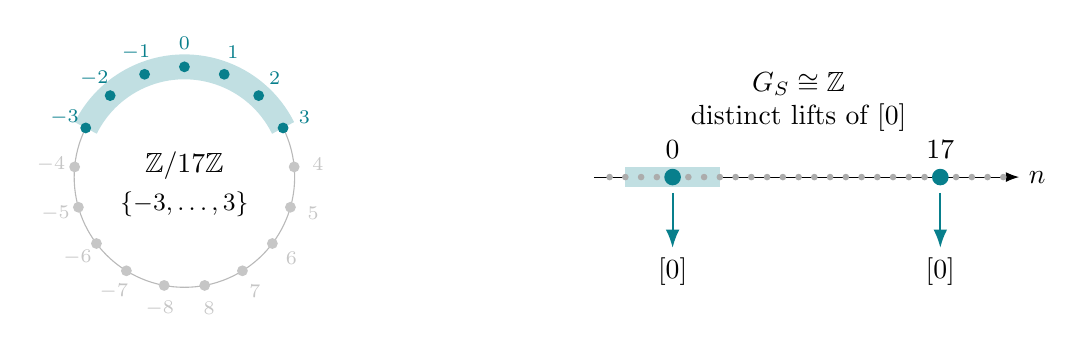
\begin{tikzpicture}[>=Latex]
\begin{scope}[xshift=-3.4cm,scale=.70]
\draw[gray!55] (0,0) circle (2);
\draw[teal!25,line width=9pt] ({90-360*3/17}:2)
arc ({90-360*3/17}:{90+360*3/17}:2);
\foreach \n in {-8,...,8}{
\ifnum\n>-4\ifnum\n<4\def\pc{teal}\else\def\pc{gray!45}\fi\else\def\pc{gray!45}\fi
\fill[\pc] ({90-360*\n/17}:2) circle (2.8pt);
\node[font=\scriptsize,text=\pc] at ({90-360*\n/17}:2.43) {$\n$};}
\node at (0,.2) {$\Z/17\Z$};
\node[font=\small] at (0,-.5) {$\{-3,\ldots,3\}$};
\end{scope}
\begin{scope}[xshift=2.8cm,x=.20cm]
\draw[->] (-5,0)--(22,0) node[right] {$n$};
\draw[teal!25,line width=7pt] (-3,0)--(3,0);
\foreach \n in {-4,...,21}{\fill[gray!65] (\n,0) circle(1.2pt);}
\foreach \n in {0,17}{\fill[teal] (\n,0) circle(3pt);
\node[above=3pt] at (\n,0) {$\n$};
\draw[->,teal,thick] (\n,-.2)--(\n,-.9);
\node[below] at (\n,-.9) {$[0]$};}
\node[align=center] at (8,.95) {$G_S\cong\Z$\\distinct lifts of $[0]$};
\end{scope}
\end{tikzpicture}
\caption{The small arc has unique small integer representatives. On the
integer cover, points differing by $17$ remain distinct even though
they project to the same residue.}
\label{fig:cover}
\end{figure}

\subsection{The lifted group records the carry}
For general $G,S$, define
\begin{equation}\label{eq:lifted-group}
G_S=\{(x,\theta)\in G\times\R^S:
\theta_\xi=\xi\cdot x\pmod1\text{ for all }\xi\in S\}.
\end{equation}
It fits into the exact sequence
\[0\longrightarrow\Z^S\longrightarrow G_S\longrightarrow G\longrightarrow0.\]
The first map is $n\mapsto(0,n)$ and the second is projection to $x$.
Lifting generators of $G$ and adjoining the coordinate generators of
$\Z^S$ proves that $G_S$ is finitely generated. It need not be
torsion-free: elements of $G$ annihilated by all of $S$ may remain
as torsion upstairs.

For the cyclic example,
\[G_S=\{([n],n/17):n\in\Z\}\cong\Z.\]
In this group,
\[([8],8/17)+([1],1/17)=([-8],9/17)\ne([-8],-8/17).\]
The second coordinate remembers which integer representative was used.
Consequently
\[
\widetilde B\bigl(([n],n/17),([m],m/17)\bigr)=\alpha nm
\]
is globally bilinear upstairs and agrees with \eqref{eq:example-form}
on the small lifts. This is the content of \JT{Example 2.3}.
The small representative map is a local map, not a global homomorphic
section $\Z/N\Z\to\Z$: such a section cannot exist when $N>1$.

\subsection{The precise algebraic black boxes}
\begin{liftlemma}
Let $G$ be finite abelian, $S\subseteq\Gh$, $0<r<1/2$, and $H$
an abelian group. If $B:\Bohr(S,r)^2\to H$ is locally bilinear,
there is a globally bilinear map $\widetilde B:G_S^2\to H$ satisfying
\[
\widetilde B((x,\theta),(y,\sigma))=B(x,y)
\quad\text{when }\norm{\theta}_\infty,\norm{\sigma}_\infty\leq
\exp(-C|S|^C)r,
\]
for an absolute $C>0$. If $B$ is symmetric, $\widetilde B$ may be
chosen symmetric.
\end{liftlemma}
This is \JT{Lemma 2.2}. It extends the form to the lifted group, with
agreement only on a smaller neighbourhood. The exponential shrink in
the rank is the source of the exponential radius in Theorem 1.6.

\begin{integrationlemma}
\leavevmode
\begin{enumerate}
\item If $A$ is a finitely generated abelian group and
$\widetilde B:A^2\to\T$ is symmetric and globally bilinear, there
exists a globally quadratic map $\widetilde\phi:A\to\T$ such that
\[
\widetilde\phi(u+v)=\widetilde\phi(u)+\widetilde\phi(v)+\widetilde B(u,v)
\quad(u,v\in A).
\]
\item If $G$ is finite abelian, $S\subseteq\Gh$, $r>0$, and
$B:\Bohr(S,r)^2\to\T$ is symmetric and locally bilinear, there
exist a radius $r'$ with
$\exp(-|S|^{O(1)})r\ll r'\leq r$ and a locally quadratic map
$\phi:\Bohr(S,r')\to\T$ satisfying
\[
\phi(x+y)=\phi(x)+\phi(y)+B(x,y)
\quad(x,y\in\Bohr(S,r'/2)).
\]
Moreover, $\phi$ has a globally quadratic lift
$\widetilde\phi:G_S\to\T$ agreeing with $\phi(x)$ whenever
$(x,\theta)\in G_S$ and $\norm{\theta}_\infty<r'$.
\end{enumerate}
\end{integrationlemma}
This is \JT{Lemma 2.4}. Its local part is the composition: lift $B$
using Lemma 2.2, integrate on the finitely generated group $G_S$, and
restrict to canonical small lifts. The next observations explain that
composition and the torsion issue; the theorem will use the two lemmas
as stated.

\subsection{Why restriction gives a locally quadratic map}
For $r<1/2$, each $x\in\Bohr(S,r)$ has a unique lift
$\widetilde x=(x,\theta_x)$ with $\norm{\theta_x}_\infty<r$.
If $x,y,x+y$ lie in this set and $3r<1$, the integer vector
$\theta_x+\theta_y-\theta_{x+y}$ has norm below one, hence vanishes.
Similarly, if all four vertices of a parallelogram lie in the set and
$4r<1$, their lifts satisfy the same parallelogram relation. On any cube
lying there, the lifted vertices consequently form an affine cube.
Restricting a global quadratic on $G_S$ therefore gives a locally
quadratic map in the full cube sense.

\subsection{Concrete primitives and even torsion}
On the integer cover, the real parabola $\alpha n^2/2$ gives
\[
\widetilde\phi(n)=\alpha n^2/2\pmod1,
\qquad
\widetilde\phi(n+m)-\widetilde\phi(n)-\widetilde\phi(m)=\alpha nm\pmod1.
\]
Restricting it to the small interval gives the required local quadratic.
The use of $\T$ as codomain is also important for torsion. On
$\Z/2\Z$, the form $B(1,1)=1/2$ has the primitive
$\phi(0)=0$, $\phi(1)=1/4$, because
$1/4+1/4+1/2=0$ modulo one. Fourth roots of unity naturally appear
even though the group has exponent two.

More generally, every bilinear form on $\Z/N\Z$ has the shape
$B([n],[m])=anm/N\pmod1$ for an integer $a$. A primitive is
\begin{equation}\label{eq:cyclic-primitive}
\phi([n])=\frac{a\,n(n-N)}{2N}\pmod1.
\end{equation}
Indeed,
\[
\phi(n+N)-\phi(n)=an\in\Z,\qquad
\phi(n+m)-\phi(n)-\phi(m)=\frac{anm}{N}\pmod1.
\]
The linear correction in \eqref{eq:cyclic-primitive} enforces periodicity
and leaves the polarisation unchanged. Thus the formula works for both
odd and even $N$. Together with the primitive on $\Z$, this explains
the integration lemma on all finitely generated abelian groups: on a
product, add the primitives on the factors and add one cross term
$B(x_i,x_j)$ for each pair $i<j$. Symmetry makes the polarisation equal
to the full form. Arbitrary division of $B(x,x)$ by two in $\T$ would
not provide this compatibility with the group relations.

\section{Completing the proof of Theorem 1.6}\label{sec:finish}
\subsection{Preserving correlation while shrinking the neighbourhood}
Start with the form and the correlation supplied by Lemma 2.6, using
$P=\Bohr(S,\rho)$. Lemma 2.4 and regular-radius selection give a
regular $\bb_1=\Bohr(S,r_1)$ and a locally quadratic $\phi$ on
$\Bohr(S,2r_1)$ with
\begin{equation}\label{eq:polarisation}
B(y,z)=\phi(y+z)-\phi(y)-\phi(z)
\quad(y,z\in\bb_1).
\end{equation}
Take $r_1$ below a sufficiently small polynomial multiple of $\rho$,
retaining $r_1\gg\exp(-\ipoly)$. Choose a second regular set
$\bb_2=\Bohr(S,r_2)$ with $r_2$ a sufficiently small polynomial
multiple of $r_1$. We can ensure \eqref{eq:sumset-ratio} for
$\bb_1,\bb_2$, and that all shifts below remain in the doubled
domain of $B$.

Directly restricting \eqref{eq:bilinear-correlation} to these tiny
sets could lose an exponential factor. Instead average its small
translations
\[(h,k)\mapsto(h+y+z,k-y),\qquad y\in\bb_1,\ z\in\bb_2.\]
Regularity controls the error, so
\begin{equation}\label{eq:shifted-final}
\abs{\E_{\substack{x\in G,\ h,k\in P\\y\in\bb_1,\ z\in\bb_2}}
b_1(x,h+y+z)b_2(x,k-y)
f(x+h+k+z)e(-B(h+y+z,k-y))}\gg\poly.
\end{equation}
Symmetry and \eqref{eq:polarisation} let us collect the phase into
terms involving $y$, $y+z$, and a single surviving $-\phi(z)$.
Expanding the phase explicitly, symmetry gives
\[
B(h+y+z,k-y)=B(h,k)-B(h,y)+B(y+z,k)-B(y,y)-B(y,z).
\]
Use $B(y,z)=\phi(y+z)-\phi(y)-\phi(z)$. With the minus sign in the
exponential, one can assign the factors explicitly:
\[
\begin{aligned}
a_{x,h,k}(y+z)&=b_1(x,h+y+z)e(-B(y+z,k)+\phi(y+z)),\\
b_{x,h,k}(y)&=b_2(x,k-y)e(B(h,y)+B(y,y)-\phi(y)-B(h,k)).
\end{aligned}
\]
The remaining factor is exactly $f(x+h+k+z)e(-\phi(z))$.
Thus no unwanted function depending only on $z$ is hidden in $b$.
After $x'=x+h+k$ and pigeonholing $h,k$, the desired factorisation holds.
In particular, after fixing $h,k$ we have
\begin{equation}\label{eq:trilinear-final}
\abs{\E_{x\in G,y\in\bb_1,z\in\bb_2}
a(x,y+z)b(x,y)f(x+z)e(-\phi(z))}\gg\poly.
\end{equation}

\subsection{Extracting the last linear phase}
\begin{lemma}[Local Fourier extraction; {\GT{Lemma 4.4}}]\label{lem:extraction}
Let $P,Q$ be nonempty subsets of a finite abelian group, let
$g:G\to\C$, and let $a,b:G\to\C$ be 1-bounded. Then
\[
\sup_{\xi\in\Gh}\abs{\E_{z\in Q}g(z)e(-\xi\cdot z)}
\geq\frac{|P|}{|P+Q|}
\abs{\E_{y\in P,z\in Q}b(y)a(y+z)g(z)}.
\]
\end{lemma}
\begin{proof}
For the final Fourier lemma let $p=|P|/|G|$, $q=|Q|/|G|$ and
$r=|P+Q|/|G|$. Extend
$F=g\mathbf1_Q$, $B=b\mathbf1_P$, $A=a\mathbf1_{P+Q}$ by zero.
Then, with the normalised transform convention,
\[
I:=\E_{y\in P,z\in Q}b(y)a(y+z)g(z)
=\frac1{pq}\sum_\xi\widehat F(\xi)\widehat B(\xi)\widehat A(-\xi).
\]
Cauchy--Schwarz and Parseval yield
\[
|I|\leq\frac{\sup_\xi|\widehat F(\xi)|}{pq}\sqrt{pr}
=\sqrt{r/p}\sup_\xi\abs{\E_{z\in Q}g(z)e(-\xi\cdot z)}.
\]
Since $r\geq p$, this implies the weaker factor $p/r$ stated in
\GT{Lemma 4.4}.
\end{proof}
Apply the lemma for each $x$ to
$g_x(z)=f(x+z)e(-\phi(z))$, $P=\bb_1$ and $Q=\bb_2$, extending
$g_x$ arbitrarily outside its required domain. By regularity,
$|\bb_1+\bb_2|\leq2|\bb_1|$. If $I_x$ denotes the inner
$(y,z)$-average in \eqref{eq:trilinear-final}, then
\[
\E_x\sup_\xi\abs{\E_{z\in\bb_2}g_x(z)e(-\xi\cdot z)}
\geq\tfrac12\E_x|I_x|\geq\tfrac12|\E_x I_x|\gg\poly.
\]
Choose a maximiser $\xi(x)$, possible because $\Gh$ is finite.
This proves the required correlation on $\bb_2$.

\subsection{Checking the quantitative conclusion}
Every rank enlargement in Lemmas 2.5--2.6 is polynomial in $1/\eta$,
as are the losses in correlation and the radius losses before
integration. Lemma 2.4(ii) contributes an exponential shrink in
$|S|^{O(1)}$, which is still of the form $\exp(-\eta^{-O(1)})$.
The final polynomial shrink from $r_1$ to $r_2$ preserves that lower
bound. Choose the final regular radius below $1/100$.
Thus
\[
|S|\ll\eta^{-O(1)},\qquad
\exp(-\eta^{-O(1)})\ll r_2\leq1/100,
\]
and the correlation is $\gg\eta^{O(1)}$. Restricting $\phi$ to
$\bb_2$ preserves local quadraticity. This proves Theorem 1.6.

\section{The finite-field model for the combinatorial step}\label{sec:finite-field}
The argument becomes geometrically simpler for $G=\F_5^n$, as explained
in \Green{Propositions 2.5--2.6}. Identify $\Gh$ with $\F_5^n$
using the standard dot product divided by five. The derivative-frequency
and energy arguments are the same. After BSG, $\Gamma'$ is a large
subset of $\F_5^{2n}$ of small doubling.

Here is the additional qualitative black box used in that model.
\begin{theorem}[Finite-field Freiman; {\Green{Proposition 1.14}}]
For a fixed prime $p$ and $K\geq1$, there is a constant $C_{p,K}$
such that every finite nonempty $A\subseteq\F_p^m$ satisfying
$|A+A|\leq K|A|$ is contained in a linear subspace $W$ with
$|W|\leq C_{p,K}|A|$.
\end{theorem}
Apply this to $\Gamma'$ (Pl\"unnecke or the standard sum--difference
inequalities convert the small difference bound to small doubling).
The resulting subspace $W\leq\F_5^{2n}$ has $|W|\leq C_\eta|G|$,
and its projection $\pi W$ onto the first factor contains at least
$c_\eta|G|$ points. Therefore
\[
|\ker(\pi|_W)|=\frac{|W|}{|\pi W|}\leq C'_\eta.
\]
Choose a vector-space complement $W_0$ to this kernel. There are only
$C'_\eta$ cosets of $W_0$ in $W$, so one coset captures a positive
$\eta$-dependent proportion of $\Gamma'$. Projection is injective on
that coset; consequently it is the graph of an affine map on an affine
subspace of $G$. On a large subset of the good increments,
\[\xi_h=Lh+\xi_0.\]
The linear part extends from its subspace to $G$ by choosing a basis.
As before, align the original correlations and absorb the affine
correction to obtain a linear frequency map.

This explains the geometry of the graph construction. For the polynomial
bounds in the stated theorem, however, the graph-refinement/Bogolyubov
argument of Section~\ref{sec:frequencies} is the relevant proof; the
qualitative constants $C_{p,K}$ above alone do not imply them. In
$\F_p^n$, a Bohr set of radius below $1/p$ is an intersection of
character kernels, hence a subspace. A locally linear map on that
subspace is simply linear. This is the model behind the local language
needed for general finite abelian groups.

\appendix
\section{The local Bogolyubov mechanism}\label{app:local-bogolyubov}
Here is a derivation of the additive-combinatorial ingredient in the
symmetry step, following the mechanism of \GT{Lemma 8.8}, with constants suppressed
but the density dependence retained.

Let $U=\Bohr(S,r)$ be regular, $d=\max(1,|S|)$,
$A\subseteq U$, and $|A|=\delta|U|$. Take a regular
$U'=\Bohr(S,r')$ with $r'\asymp\delta r/d$, sufficiently small that
the regularity error is at most $\delta/2$. Averaging over translates
$x+U'$, $x\in U$, gives some $x_0$ for which
\[A'=A\cap(x_0+U'),\qquad |A'|\geq(\delta/2)|U'|.\]
Use $\beta=|U|/|G|$, $\beta'=|U'|/|G|$ and normalised convolution.
The function $\mathbf1_A*\mathbf1_{A'}$ is supported in
$x_0+U+U'$, of size at most $2|U|$. Cauchy--Schwarz and Parseval give
\[
F(0):=\sum_\xi|\widehat{\mathbf1_A}(\xi)|^2
                         |\widehat{\mathbf1_{A'}}(\xi)|^2
\geq\frac{\delta^4\beta(\beta')^2}{8}.
\]
The function
$F=\mathbf1_A*\mathbf1_{A'}*\mathbf1_{-A}*\mathbf1_{-A'}$
is supported in $2A-2A$. Define
\[R=\{\xi:|\widehat{\mathbf1_{A'}}(\xi)|\geq
                       (\delta^{3/2}/8)\beta'\}.\]
The Fourier mass outside $R$ is at most
$\delta^4\beta(\beta')^2/64$. Therefore, whenever
$\norm{\xi\cdot x}_\T<1/10$ for every $\xi\in R$,
\[
F(x)\geq\tfrac12F(0)-2\sum_{\xi\notin R}
|\widehat{\mathbf1_A}(\xi)|^2|\widehat{\mathbf1_{A'}}(\xi)|^2>0.
\]
It remains to enforce these possibly numerous frequency constraints with
only polynomially many new characters. That is the role of the local
Bessel inequality.

\textbf{Local Bessel input, exact claim.}
If $V=\Bohr(S,s)$ is regular, $E\subseteq V$, and
\[\mathcal R=\{\xi:|\widehat{\mathbf1_E}(\xi)|\geq t|V|/|G|\},\]
then, for $0<\theta,t\leq1$, there exist at most $2/t^2$ frequencies
$\xi_1,\ldots,\xi_m$ such that each $\xi\in\mathcal R$ satisfies
\[\sup_{x\in\Bohr(S,\theta s)}
\norm{(\xi-\xi_j)\cdot x}_\T\leq2^{16}\theta d/t^4
\quad\text{for some }j.\]
This is \GT{Corollary 8.7}. To see its proof, choose a maximal set of
frequencies separated by $q=2^{16}\theta d/t^4$ in this seminorm.
Local Fourier decay (applied to differences of characters) bounds the
off-diagonal inner products on $V$ by
$2^6(\theta d/q)^{1/2}\leq t^2/4$.
Choose phases aligning the correlations with $\mathbf1_E$.
Cauchy--Schwarz gives
\[t^2m^2\leq\E_{x\in V}\abs{\sum_{j=1}^m c_j e(\xi_j\cdot x)}^2
\leq m+\tfrac12t^2m^2.\]
Hence $m\leq2/t^2$. Maximality ensures that these frequencies cover
the large spectrum in the displayed seminorm. This derives the input
from the local Fourier-decay lemma, rather than invoking an additional
structural theorem.

Apply it to $E=A'-x_0\subseteq U'$; translation preserves Fourier
magnitudes. With $t=\delta^{3/2}/8$, there are
$m=O(\delta^{-3})$ representative frequencies. Set
$\theta=c\delta^6/d$ sufficiently small that the approximation error
is below $1/20$. On a Bohr set enforcing $\norm{\xi_j\cdot x}<1/20$
and the old constraints at radius $\theta r'$, every frequency in $R$
has circle norm below $1/10$. Thus the positive-convolution argument
puts this Bohr set inside $2A-2A$.

Since $r'\asymp\delta r/d$, this elementary tracking yields the slightly
weaker but fully sufficient radius $c\delta^7r/d^2$, with
$O(\delta^{-3})$ new characters. \GT{Lemma 8.8} states the sharper
$c\delta^6r/d$ radius in Lemma~\ref{lem:local-bogolyubov}. That
sharper statement can be used as a black box; the argument here proves
a polynomial-radius version from scratch, which is all the symmetry
argument needs. In particular, no
global density such as $|A|/|G|$ enters the rank bound.

\section{Conventions when comparing the original papers}\label{app:conventions}
The following points help match the preceding argument with its sources.
\begin{itemize}
\item The numbered statements Theorem 1.6 and Lemmas 2.2, 2.4, 2.5,
2.6 are those of Jamneshan--Tao. Green's lecture notes have their own
Proposition 2.5; it is a different statement.
\item In the printed Example 2.3, an integer representative map is
described as a homomorphic section. A homomorphism $\Z/N\Z\to\Z$
is zero for $N>1$, so the local representative interpretation in
Section~\ref{sec:algebra} is the one used here.
\item Green--Tao's Propositions 9.1 and 9.3 write the graph as
$(h,2M(h))$. The implicit odd-order assumption is identified in
\JT{Lemma 2.5, footnote 6}. Constructing $(h,M(h))$ directly removes
it. Likewise the final doubling manoeuvre in their symmetry argument
is omitted.
\item The lift in Green--Tao's Proposition 9.1 belongs to
$2\Gamma''-2\Gamma''$, not $2H''-2H''$, as JT footnote 7 notes.
For two pair sums we use the graph property of $4\Gamma''-4\Gamma''$;
the larger set $8\Gamma''-8\Gamma''$ is only known to have trivial
zero fibre.
\item In the final Fourier display of the printed JT proof, the radius
is labelled $\rho_1$. Applying the stated Fourier lemma to the preceding
trilinear average gives the coefficient on the $z$ domain
$\Bohr(S,\rho_2)$. Section~\ref{sec:finish} consistently uses this
smaller set, which satisfies every bound required by Theorem 1.6.
\item The December 2023 correction on the
\href{https://arxiv.org/abs/math/0503014}{Green--Tao arXiv record}
concerns Proposition 3.2, a global extension assertion not used here.
Our algebraic extension is JT Lemma 2.2 on $G_S$.
\end{itemize}

\begin{thebibliography}{Green}
\raggedright
\bibitem[JT]{JT}
A. Jamneshan and T. Tao,
\emph{The inverse theorem for the $U^3$ Gowers uniformity norm on arbitrary
finite abelian groups: Fourier-analytic and ergodic approaches},
Discrete Analysis 2023:11 (2023), 48 pp.
\href{https://doi.org/10.19086/da.84268}{doi:10.19086/da.84268};
\href{https://arxiv.org/abs/2112.13759v3}{arXiv:2112.13759v3}.
\bibitem[GT]{GT}
B. Green and T. Tao,
\emph{An inverse theorem for the Gowers $U^3(G)$ norm},
Proc. Edinb. Math. Soc. (2) \textbf{51} (2008), 73--153.
\href{https://doi.org/10.1017/S0013091505000325}{doi:10.1017/S0013091505000325};
\href{https://arxiv.org/abs/math/0503014v4}{arXiv:math/0503014v4},
including the December 2023 correction.
\bibitem[Green]{Green}
B. Green,
\emph{Montr\'eal lecture notes on quadratic Fourier analysis},
\href{https://arxiv.org/abs/math/0604089v2}{arXiv:math/0604089v2} (2007).
\end{thebibliography}
\end{document}
